\documentclass[12pt]{article}

% Set border
\usepackage[margin=1in]{geometry}

% Used for improving math typesetting and including certain symbols
\usepackage{amsmath}
\usepackage{physics}

% Use pictures and graphics
\usepackage{graphicx}
\graphicspath{ {images/} }

% Custom link colors
\usepackage{xcolor}
\usepackage{hyperref}
\hypersetup{
  colorlinks,
  linkcolor={black},
  citecolor={black},
  urlcolor={blue!80!black}
}

% Allow text to wrap around figures
\usepackage{wrapfig}

% Auto begin/end quotes (instead of having to use `` ")
\usepackage [autostyle, english = american]{csquotes}
\MakeOuterQuote{"}

% Used to include certain symbols (including /degree)
\usepackage{gensymb}

% Code listings/highlighting
\usepackage{minted}[cache=false]

% TITLE ----------

\title{CMPU-250: Final Project Write-up \\
  \large Autonomous Robotics Design Competition Simulation}
\date{May 2018}
\author{George Witteman}

% DOCUMENT -------

\begin{document}

\maketitle

\begin{abstract}
  For my final project I chose to design and implement an agent-based model of Vassar's Autonomous Robotics Design Competition class in the Cognitive Science department. This model simulates two robots in the arena using a slightly modified version of the rules. The model is validated by testing individual functions for correctness, as well as visually testing that the behavior is correct. Finally, the model is evaluated using hypothesis testing to test assumptions about the competition, such that the addition of a camera will improve the efficiency of the robots or that increasing the velocity or rotation speed of the robot will increase it's score.
\end{abstract}

\section{Introduction}

Vassar's Autonomous Robotics Design Competition is a class in the Cognitive Science department that gives students the opportunity to create robots designed to complete a specific task. In the course, students work in teams and, using Arduinos, foam core, 3D printers, \href{http://charmedlabs.com/default/pixy-cmucam5/}{Pixy} camera, and various other electronics, build a robot that competes with the other team's robot to fulfill a certain task as best as possible within a given time frame.

This year, the goal of the competition is for teams to create a robot that gains the best score by collecting blocks of it's own quadrant's color into it's home quadrant, and removing blocks of other colors from it's home quadrant. There is also a sabotage element that can be implemented by moving blocks that are not the opponents color into the opponents quadrant.

During the actual competition, three of the four teams used a strategy that collected one block at a time and moved it to an appropriate quadrant. My team decided that a collection strategy would prove more beneficial, since it could rely less heavily on the camera if that proved to not be easy to implement. Since we were not able to fully finish completing our robot, I wanted to build this model in order to test some of the theories we had about why our robot would perform well. I tried to build this model as closely as possible to the version that we created, including the camera function.

This model includes a visualization of the arena that can be seen over time. See Figure \ref{fig:arena-1} for an example of this. In this figure, you're able to see the arena including the outer and quadrant boundary lines, blocks, and robots. The two robots are represented by rectangles with a triangle in the middle indicating their direction. The robots camera is also represented by drawing it's field of view as a mostly transparent semi-circle in front of the robot. The time that the simulation has been running for is indicated in the title of the plot, and when the simulation finishes the points for each team and winner is displayed in the MATLAB command window.

\begin{figure}[hbt]
  \center
  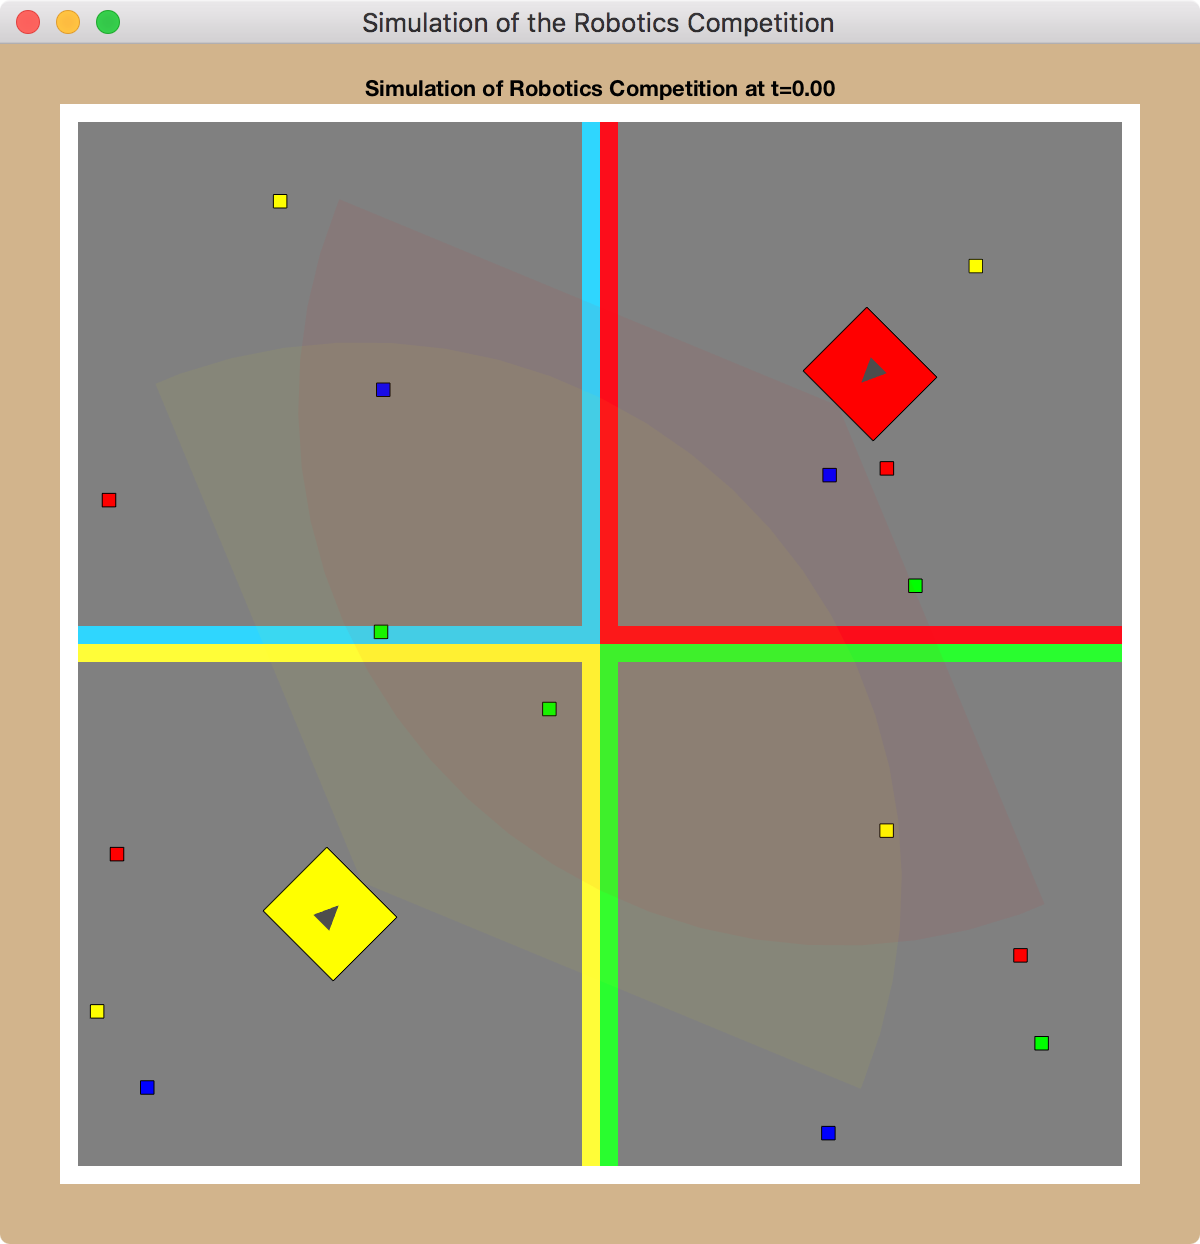
\includegraphics[width=0.45\textwidth]{images/arena-1.png}
  \caption{An example starting simulation state. You can see two robots (red and yellow) and twelve blocks spread out evenly through the four quadrants. The direction the robot is facing as well as it's camera's field of view is also represented.}
  \label{fig:arena-1}
\end{figure}

\section{Simplifying Assumptions}
\begin{itemize}
  \item Robots can reach their full velocity and come to a stop instantly.
  \item All robots are identical in their software and hardware implementations.
  \item Blocks cannot be pushed, only collected or ignored.
  \item Placing blocks into the quadrant of the opponent or removing other color blocks from the home quadrant is insignificant. That is, being able to collect home color blocks and bringing them back to the home quadrant is the most important thing.
  \item The robot's cameras are perfect accurate within their field of view.
  \item The sorting mechanism is perfect. That is, blocks are either completely ignored (not moved at all) or collected into the chamber with 100\% accuracy.
  \item The rotation of the blocks is insignificant.
  \item Robots can run over each when backing up, but not when going forward. I chose to make this assumption in order to prevent bots from getting stuck when they are backing up. This would mostly happen when $dt$ is low, and does not seem to impact the results of a simulation.
\end{itemize}

\section{Code Validation}
There were two main strategies that I used to validate my code. First, I tested individual functions by manually building instances of the classes and running tests on specific functions. Second, I tested the system as a whole by running multiple random simulations using the same and differing parameters and looking at the results to make sure that things were running as expected.

\subsection{Individual Function Tests}
My first strategy for testing my code was to test individual methods by creating test instances of classes, manually setting parameters, and then testing the output of the methods using inputs where I had manually calculated the output.

For example, I validated the validity of the method \texttt{inFieldOfView} on the \texttt{Camera} class by creating a new instance of the \texttt{Camera} in the command window with the command \texttt{c = Camera(5, 135, 'red')}. Then, I tested the function with a number of different points. For example, the camera should be able to see a block 1 foot in front of it, so to test that I used the command \texttt{c.inFieldOfView(0,0,0,1,0)} which returned \texttt{1}, the expected output. Another test that I ran is for blocks that should not be in the field of view. One command I used to test that was \texttt{c.inFieldOfView(0,0,0,-1,0)} which returns \texttt{0}, since the block is behind the camera position.

I did a variety of similar tests on many methods as I was developing. I would check that the results were as expected, but I would also check to make sure error cases were also handled in ways that made sense. For example when testing the \texttt{Camera.getAngleOffCenter()} method (see Listing \ref{listing:getAngleOffCenter}), I tested that the function worked for values behind the camera as well as in front of it.

\subsection{Visual System Tests}
The second strategy that I used to validate my code's accuracy was by doing visual tests. After developing individual class methods (or even just small blocks of code within a method), I would run the simulation as a whole to see the result.

One place where I used this while developing was the \texttt{Camera.getAngleOffCenter()} method (see Listing \ref{listing:getAngleOffCenter}). This method is supposed to find the angle that the input point is off the center axis of the camera. In order to find this angle it creates two lines. One line is from the camera origin to 1 unit straight forward, and the other line is from the camera origin to the point of the object. We then calculate the angle between those two lines.

When developing this function, I wanted to make sure that the lines were accurate, since I was using some trigonometry in order to calculate a point. In order to do this, I added a debug flag (\texttt{Camera.Debug}) to the constants for the \texttt{Camera} class, and then plotted the two lines if the flag is set to \texttt{true}. I could then also print out the angle that is getting returned and do a visual check to make sure that the  angle matches what I would visually expect for the two lines. This allowed me to catch a subtle error which resulted in an error checking case being added to the function (see lines 17-20 in Listing \ref{listing:getAngleOffCenter}).

Another example where I used visual testing was in the block collection code. After adding code to check collect blocks as a robot runs over it, I confirmed the validity of this feature by adding code to display the blocks that a robot has in it's chamber, and testing that when a block got added to the chamber, it was also removed from the arena.

\begin{listing}[ht]
\begin{minted}[linenos]{matlab}
function ang = getAngleOffCenter(cam_x, cam_y, cam_R, obj_x, obj_y)
  %GETANGLEOFFCENTER
  % Calculate the angle of the object relative to the center
  % axis of the camera.
  cam_x2 = cos(deg2rad(cam_R)) + cam_x;
  cam_y2 = sin(deg2rad(cam_R)) + cam_y;
  
  if Camera.Debug
    plot([cam_x cam_x2], [cam_y cam_y2]);
    plot([cam_x obj_x], [cam_y obj_y]);
  end
  
  % Find the angle between the two lines created by the points
  ang = rad2deg(atan2(obj_y-cam_y, obj_x-cam_x) - ...
    atan2(cam_y2-cam_y,cam_x2-cam_x));
  
  % Correct for error
  if ang > 180
    ang = ang - 360;
  end
end
\end{minted}
\label{listing:getAngleOffCenter}
\caption{The \texttt{Camera.getAngleOffCenter()} method.}
\end{listing}

\section{Hypothesis Tests}
The following section describes some different hypothesis that I was able to test using the model. 

\subsection{Camera Effectiveness}
\textit{Hypothesis}: The addition of the camera allows robots to collect more blocks in a shorter amount of time. In general, the addition of the camera will increase the score for the robot as opposed to roaming randomly.

To test this hypothesis I ran a 5 simulations of the competition with the camera and without the camera and averaged the resulting scores for each robot. The average score across both robots in the simulations without the camera is 6, and the average score across both robots in the simulations \textit{with} the camera is 10. That means that robots with the camera scored the maximum amount of points possible ($(3 \times 10) - (2 \times 1) = 10$) in each round. This shows that there is a significant advantage to having the camera. 

\subsection{Camera Field of View}

\end{document}